\documentclass[compress]{beamer}

\usepackage[utf8]{vntex}
\usepackage{longtable}
\usepackage{amsmath}
\usepackage{amsmath}
\usepackage{amsfonts}
\usepackage{amssymb}
\usepackage[utf8]{inputenc}
\usepackage[absolute,overlay]{textpos}

\usepackage{listings}
\lstset{
	language = Java,
	frame = single,
	tabsize = 3
}

\usetheme{Warsaw}
%\usetheme{Antibes}
%\usecolortheme{spruce}
%\setbeamercolor{structure}{fg=cyan!90!blue}

\expandafter\def\expandafter\insertshorttitle\expandafter{%
    \insertshorttitle\hfill%
    \insertframenumber\,/\,\inserttotalframenumber}
      
\AtBeginSection[] % Do nothing for \section*
{
\begin{frame}
\tableofcontents[currentsection]
\end{frame}
}
\AtBeginSubsection[] % Do nothing for \section*
{
\begin{frame}
\tableofcontents[currentsection, currentsubsection]
\end{frame}
}

\title[Mạng Google Inception]{Mạng Google Inception trong bài toán phân loại} 

\author[Nguyễn Tuấn Đạt, Đặng Quang Trung, Phan Anh Tú]{
Sinh viên thực hiện\\
Nguyễn Tuấn Đạt - 20130856\\
Đặng Quang Trung - 20134145\\
Phan Anh Tú - 20134501 \\[0.4cm]
Giảng viên \\
TS. Đinh Viết Sang 
}

\begin{document} 
\begin{frame}
\titlepage
\end{frame} 
  
\begin{frame}{Nội dung trình bày}
\tableofcontents
\end{frame}

\section{Google Inception}
\subsection{Inception Module}
\begin{frame}{Inception Module naive version}
\begin{itemize}
\onslide<1->{\item Thay vì nhìn dữ liệu theo 1 cách ở mỗi tầng thì sẽ nhìn dữ liệu theo nhiều cách}
\onslide<2->
\begin{figure}[H]
%\centering
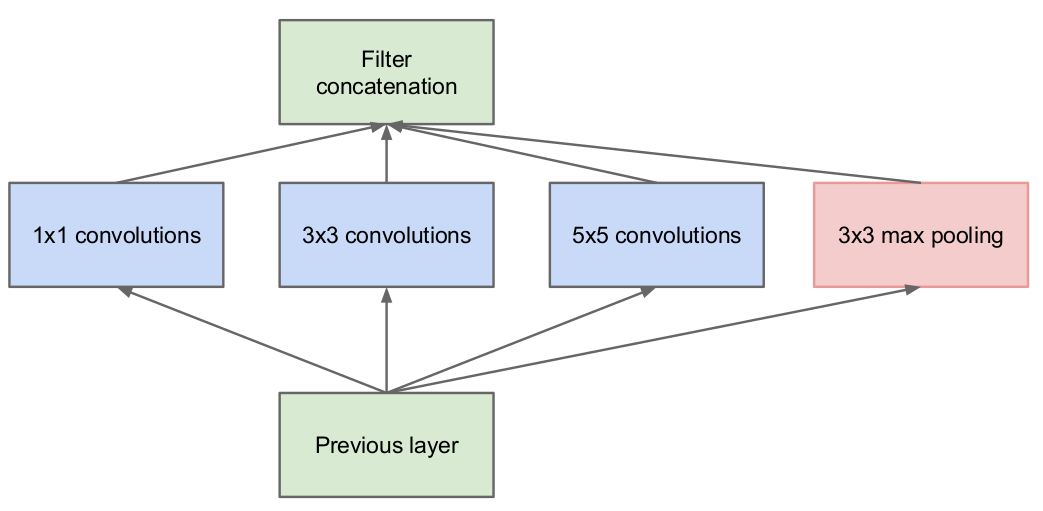
\includegraphics[scale=0.25]{inception_naive.png}
\end{figure}
\item Output của các tầng $1 \times 1$, $3 \times 3$, $5 \times 5$ là $H \times W \times C_1$, $H \times W \times C_3$, $H \times W \times C_5$  \onslide<3-> $\rightarrow$ output $H \times W \times (C_1+C_3+C_5)$

\end{itemize}
\end{frame}


\begin{frame}{Inception module với kỹ thuật giảm chiều}
\begin{itemize}
\onslide<1->{\item Để giảm chi phí tính toán, trước khi tính toán với các filter lớn ($3\times 3$ và $5 \times 5$) sử dụng các filter kích thước $1 \times 1$ để giảm chiều dữ liệu sẽ giúp cho giảm chi phí tính toán}
\onslide<2->{
\begin{figure}[H]
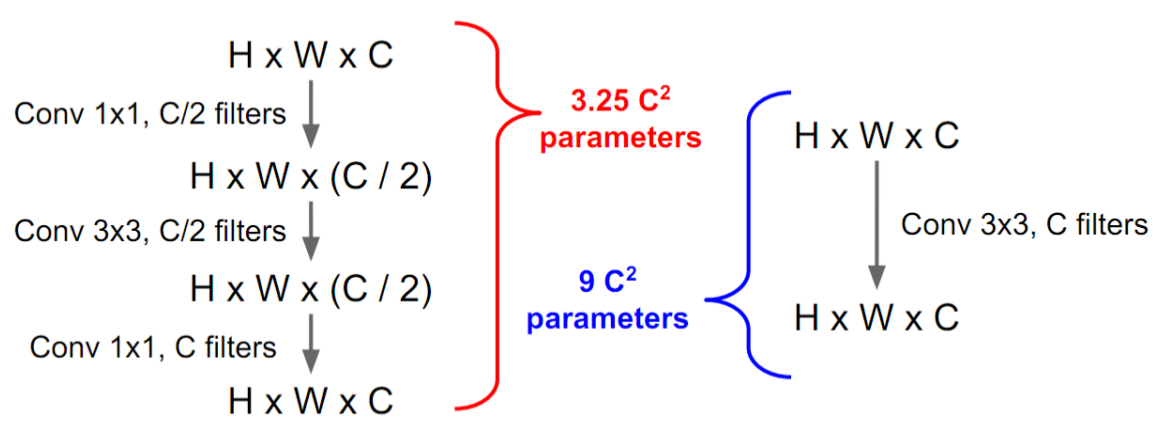
\includegraphics[scale=0.3]{reduce_1x1.png}
\end{figure}}
\end{itemize}
\end{frame}

\begin{frame}{Inception module với kỹ thuật giảm chiều}
\begin{figure}[H]
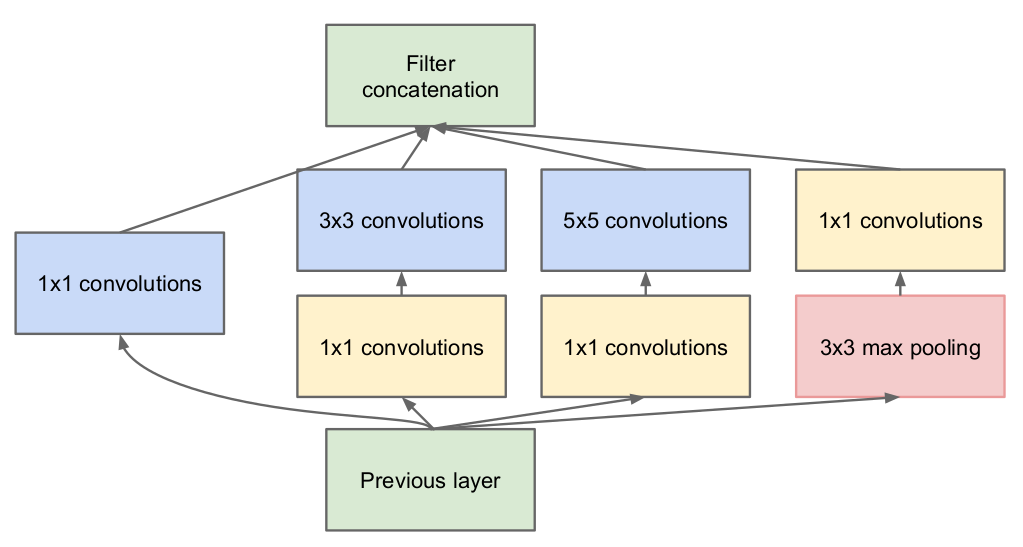
\includegraphics[scale=0.33]{inception_reduce.png}
\end{figure}
\end{frame}

\subsection{Cải tiến Inception Module}
\begin{frame}{Phân rã tầng convolution}
\begin{itemize}
\onslide<1->{\item Đặt 2 tầng Convolution (với kích thước filter mỗi tầng là $3 \times 3$ và stride là 1) cạnh nhau} 
\onslide<2->{\item Mỗi neuron thuộc tầng convolution thứ 2 sẽ nhìn vào một vùng kích thước $5 \times 5$ trong khối đầu vào của tầng thứ convolution thứ nhất} 
\onslide<3->{\begin{figure}[H]
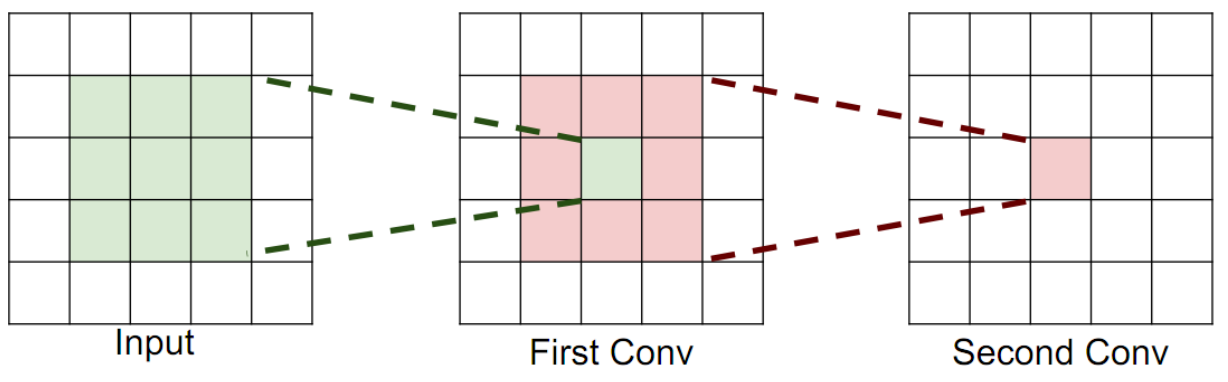
\includegraphics[scale=0.33]{2conv3x3.png}
\end{figure}}
\end{itemize}
\end{frame}

\begin{frame}{Hiệu quả của việc phân rã}
\begin{itemize}
\onslide<1->\item Một khối đầu vào có kích thước $H \times W \times C$ 
\begin{itemize}
\onslide<2->\item Một tầng convolution có $C$ filter kích thước $5 \times 5$ (với stride = 1 và padding để bảo toàn kích thước đầu vào) 
\begin{itemize}
\onslide<3->\item Số lượng tham số sẽ là: $C \times (5 \times 5 \times C) = 25C^2$ 
\onslide<4->\item Khối lượng tính toán là: $(H \times W \times C) \times (7 \times 7 \times C) = 25HWC^2$ 
\end{itemize}
\onslide<2->\item 2 tầng convolution có $C$ filter kích thước $3 \times 3$ ở mỗi tầng (với stride = 1 và padding để bảo toàn kích thước đầu vào) 
\begin{itemize}
\onslide<3->\item số lượng tham số sẽ là : $2 \times C \times (3 \times 3 \times C) = 18C^2$
\onslide<4->\item khối lượng tính toán là: $2 \times (H \times W \times C) \times (3 \times 3 \times C) = 18HWC^2$
\end{itemize}
\end{itemize}
\onslide<5-> \textbf{Phân rã 1 tầng $3\times 3$ thành 2 tầng $2 \times 2$ ???}
\end{itemize}
\end{frame}

\begin{frame}{Phân rã $2\times 2$ ??} 
\begin{itemize}
\onslide<1->\item Khối đầu vào có kích thước $H \times W \times C$ 
\begin{itemize}
\onslide<2->\item 2 tầng convolution có $C$ filter kích thước $2 \times 2$ (với stride = 1 và padding để bảo toàn kích thước đầu vào) 
\begin{itemize}
\onslide<3->\item Số lượng tham số sẽ là: $2 \times C \times (2 \times 2 \times C) = 8C^2$ 
\onslide<4->\item Khối lượng tính toán (số lượng phép toán) là: $2 \times (H \times W \times C) \times (2 \times 2 \times C) = 8HWC^2$
\end{itemize}
\onslide<2->\item 1 tầng convolution có $C$ filter kích thước $1 \times 3 $ + 1 tầng convolution có $C$ filter kích thước $3 \times 1$ (cả 2 tầng đều có tham số stride = 1 và padding để bảo toàn kích thước đầu vào)
\begin{itemize}
\onslide<3->\item Số lượng tham số là: $C \times 1 \times 3 \times C+ C \times 3 \times 1 \times C = 6C^2$ 
\onslide<4->\item khối lượng tính toán là: $(H \times W \times C) \times (1 \times 3 \times C) + (H \times W \times C) \times (3 \times 1 \times C) = 6HWC^2$
\end{itemize}
\end{itemize}
\end{itemize}
\end{frame}

\subsection{Inception v4}
\begin{frame}{Kiến trúc Inception v4}
\begin{figure}[H]
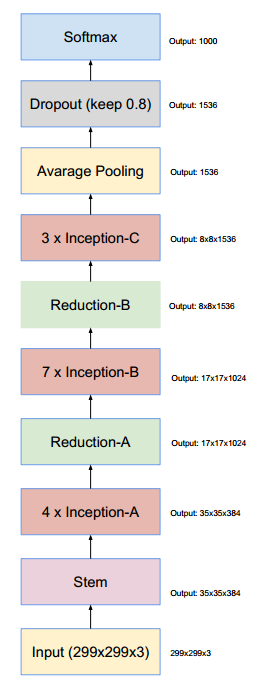
\includegraphics[scale=0.3]{inceptionv4.png}
\end{figure}
\end{frame}

\begin{frame}{Inception-A}
\begin{figure}[H]
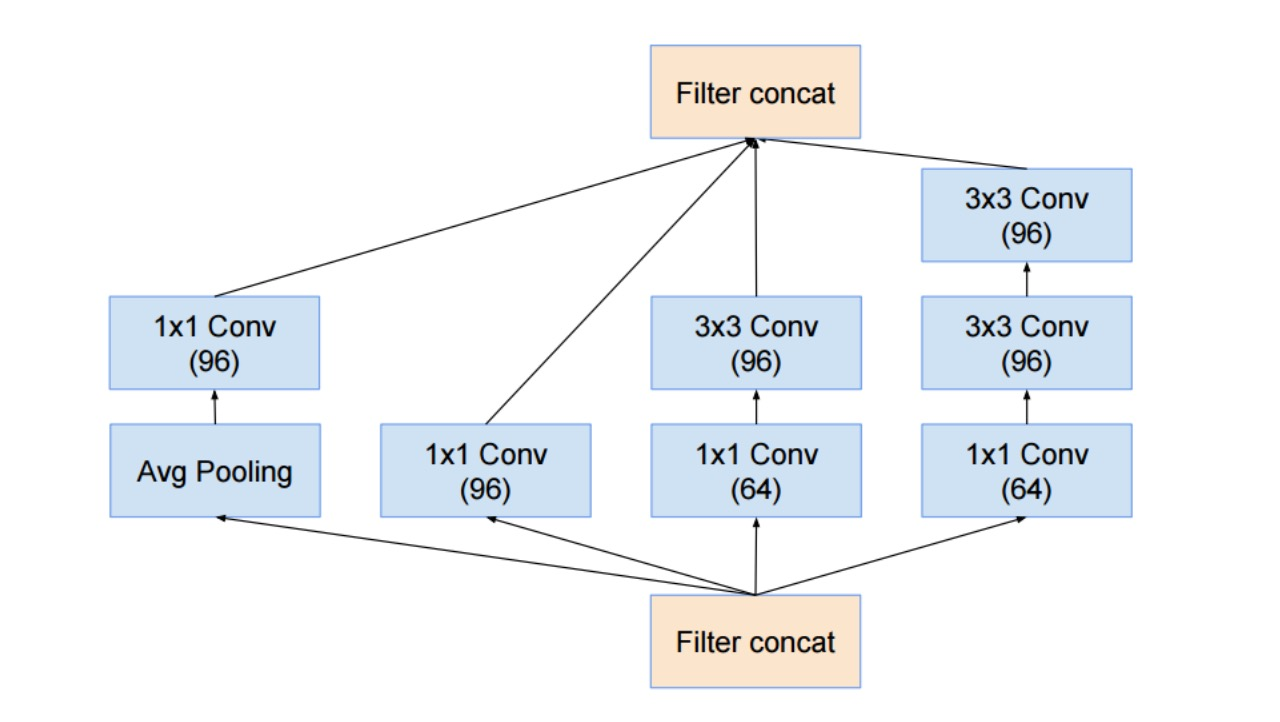
\includegraphics[scale=0.29]{inceptionA.jpg}
\end{figure}
\end{frame}

\begin{frame}{Inception-B}
\begin{figure}[H]
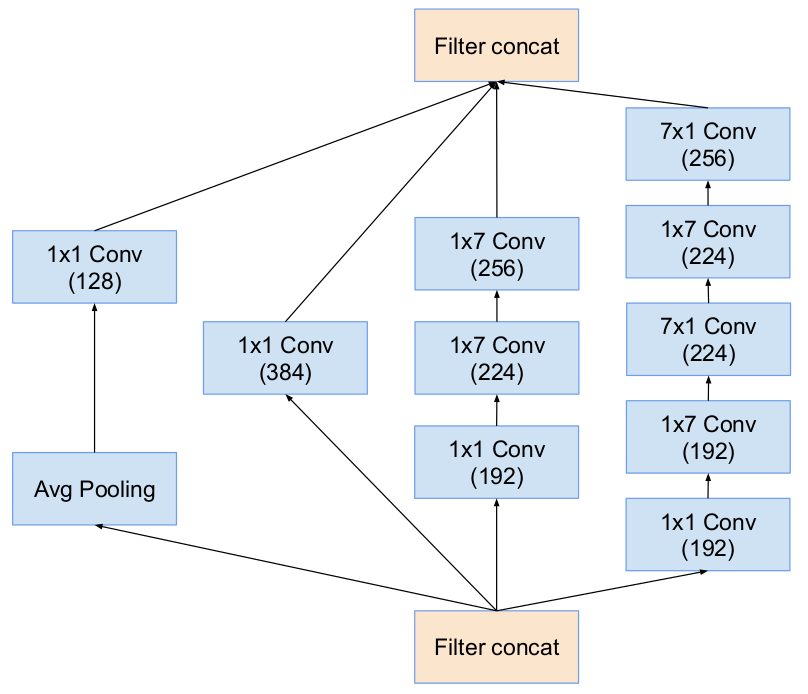
\includegraphics[scale=0.3]{inceptionB.png}
\end{figure}
\end{frame}

\begin{frame}{Inception-C}
\begin{figure}[H]
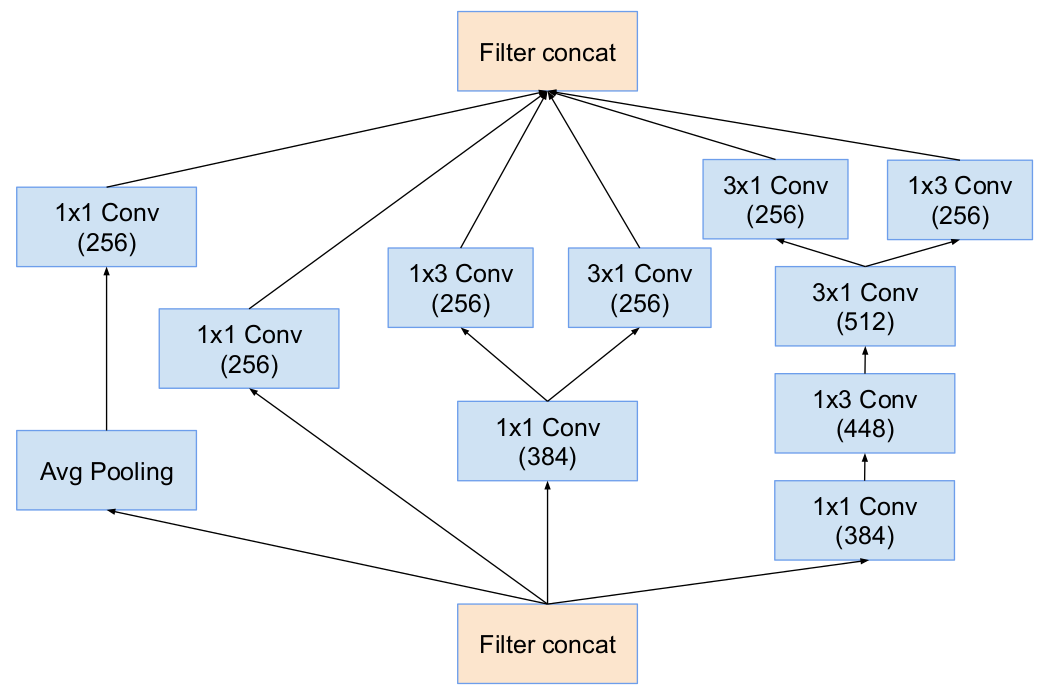
\includegraphics[scale=0.29]{inceptionC.png}
\end{figure}
\end{frame}

\begin{frame}{Reduce-B}
\begin{figure}[H]
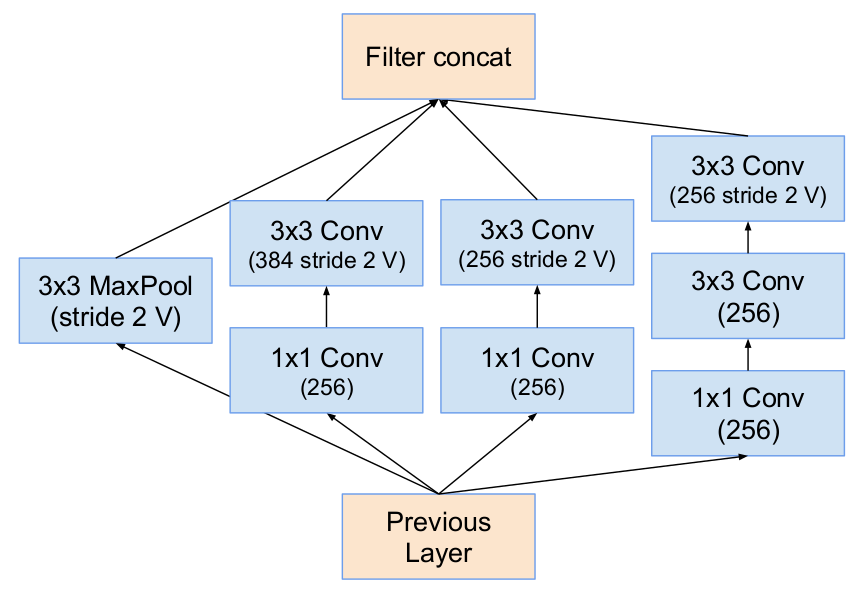
\includegraphics[scale=0.3]{reduceB.png}
\end{figure}
\end{frame}


\end{document}
